\section{Git operations}
In this section we explore some of the git operations. We try to do
so, in a different way, if comparing with other manuals. Normally the
manuals we see around just explain how to perform an operation. We
try to go further, so in this manual, we have divided our operations in
three parts. In the first part, we give a description about the
operation. In the second part, we give the pre-conditions, or in other
words, we explain in which conditions the operations can be performed.
Finally, in the last part of each operation, we show what is the
result of perform such operation.

\subsection{Add and Remove}
The operations add and remove are used to add and remove content from
index. As we have said before the index contains all the files and
contents to be added on the next commit.\\

\emph{Git} add does not refer directly to the file. Instead it is like
a map from file to content. If we have a file on the index and we
modify it on the working directory, for this modification to be visible
on the next commit, the file has to be added again to the index.\\

The remove operation removes a file from index, so it will not be
present if we perform a commit exactly after the remove. The removed
file besides of being removed from index, it will also be removed from the 
working directory (if it is still exists there).

\subsubsection{Pre requisites}
The add operation has only one pre-condition. The file has to be in
the working directory. It means that a file that is
on the working directory, can be always added to index.

Relatively to the remove operation there are a few conditions that
have to be satisfied for the remove operation be performed, which are: 
\begin{itemize}
\item The file that is being removed is currently in index;
\item The file that is being removed is in the previous commit, exactly with the same
content.
\end{itemize}

The first restriction is quite obvious. It is not possible to remove
a file if it does not exists. The last restriction exists, to avoid
the accidental deletion of file's contents. It is possible to have a
file in index with a certain content that does not exists in the
repository and since the remove operation removes the file from the index
and from the working directory, the content would be lost.  

\subsubsection{Result}
After performing the add operation there is something that will be
always observed. The file will be in index. Besides, if the file was
marked as not merged then the mark goes away. More details about
merged and unmerged files will be given later.\\

The result from performing the remove operation is that the file is
not anymore in the index. Also here the file will not be marked as
unmerged anymore.

\subsubsection{Examples}

The figure \ref{fig:add1}, shows a simple case of adding a file to the index. \\
It can be seen, that no changes are made on the repository or in the working
directory, just in the index that will contain the new file.

\begin{figure}[!h]
   \centering
   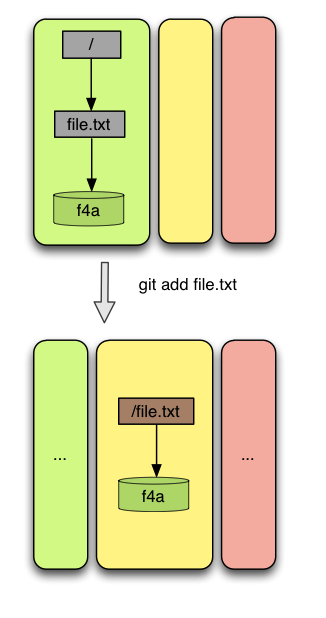
\includegraphics[width=0.4\textwidth]{images/add1.png}
   \caption{Adding a file}\label{fig:add1}
\end{figure}

Figure \ref{fig:update1}, contains the case of updating the content of a file.
\\
Assuming that the file is already in the index, changing it's content in the 
working directory, will not change the content in the index. We need to 
explicitly add the file with the new content in the index. \\ 

Now for the remove operation. Figures \ref{fig:remove1},\ref{fig:remove2} 
show a simple case of
removing a file of the index, as the reader can see the file will be
removed from the index, but also from the working directory, if it's still
there. The repository stays the same.

\begin{figure}[!h]
   \centering
   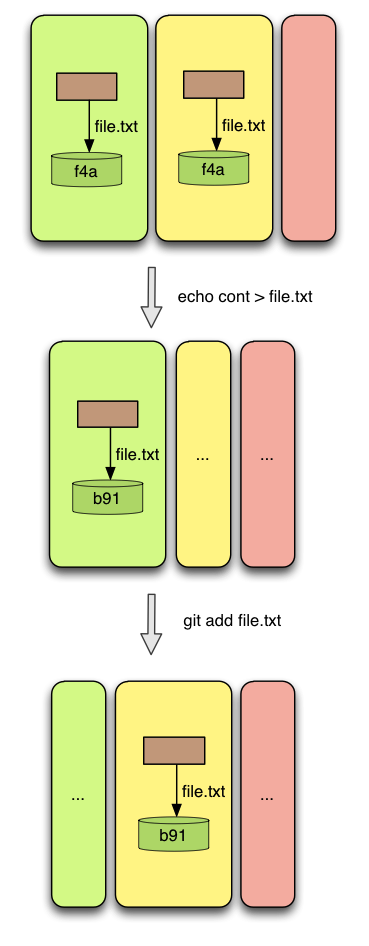
\includegraphics[width=0.5\textwidth]{images/update1.png}
   \caption{Updating a file}\label{fig:update1}
\end{figure}

\begin{figure}[!h]
   \centering
   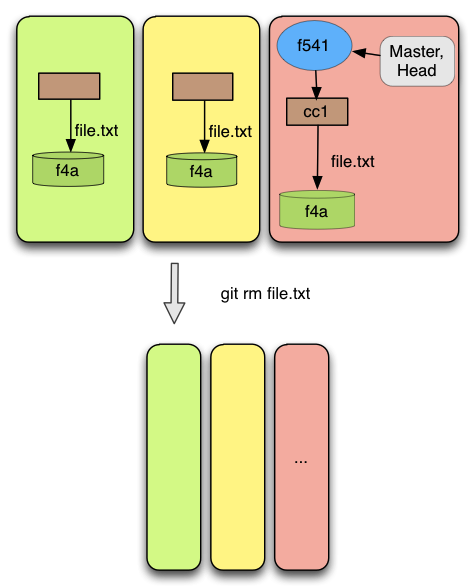
\includegraphics[width=0.6\textwidth]{images/remove1.png}
   \caption{Removing a file}\label{fig:remove1}
\end{figure}

\begin{figure}[!h]
   \centering
   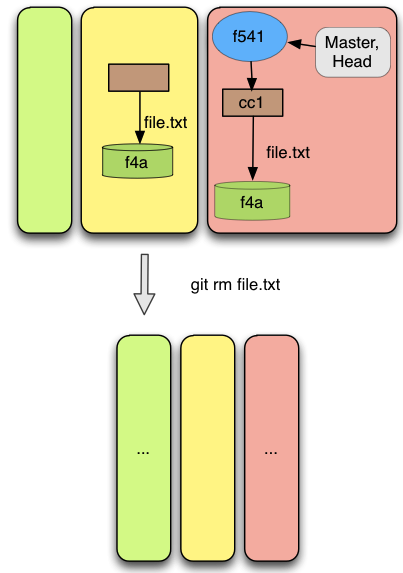
\includegraphics[width=0.6\textwidth]{images/remove2.png}
   \caption{Removing a file (alternative)}\label{fig:remove2}
\end{figure}



\subsection{Commit}
The commit operation takes the current index and builds a commit
object. Basically it takes the files from the index, builds a
structure using trees and blobs objects and creates a new commit
object pointing to the tree that corresponds to the project's root
directory. This commit object will have as parent the current commit,
the commit pointed by the branch indicated in the HEAD.
When the first commit is created, a branch called "master" will be created
and it will be marked as the current branch, or in other words, it
will be indicated by HEAD. Also, the first commit of the repository
is called a Root Commit, because it has no parents.

\subsubsection{Pre requisites}
There are three pre-conditions that are required to perform this
operation:
\begin{itemize}
   \item The index is not empty;
   \item The commit object that will be created is different from the
   current commit;
   \item There are not unmerged files.
\end{itemize}
The first pre-condition is obvious, because if we do not have files in
the index, there is anything to commit.\\

The second condition says basically
that we cannot have two commits objects pointing to the same
tree object in a row, or in other words, if we have the same files and
the same content in the index and in the current commit, a commit
operation cannot be performed. \\

The last condition just says that it is not possible to perform a
commit, if there are unmerged files in index. As we have said before,
we will speak about this later.

\subsubsection{Result}
The result of performing a commit can be different if it is the first
commit or if there are already some commit in th repository. 
We start by exposing the observed result when the first commit is
being performed and then we show the case when there are already some
commit in the repository. In the end we show some properties that are
observed in both cases.\\

The first commit object that is being created is a commit with no
parent. It means that it does not have a parent. There cannot be branches
at this moment, because they cannot point to any commit, as there are none to be
pointed, so a new branch called "master" is created. This branch is going to be pointing to 
the commit that has been created. Also the HEAD, that previously was 
not defined will identify this "master" branch.\\

When there are already some commit in the repository, then it is
guaranteed that there are at least one branch and the HEAD is
identifying some existing branch. The branch that is identified by the
HEAD, is pointing now to the commit created. This commit have now as
parent the previous commit (the commit pointed by the branch
identified by the HEAD), unless it is a result from a merge. In this
case the commit must have two parents. The previous commit and the
branch that is being merged.\\

The common properties that are observed are that all the files and
content that were in the index, are now in the current commit with the
structure from the file system. For this new blobs and trees were
probably created. The index keeps exactly the same content.

\subsubsection{Examples}

The figure \ref{fig:commit1} shows as typical process where there are added
some files to the index and then is done a commit. As can be seen the new commit
reflects, the structure of the index at that point. Also, because the two files
in the index have the same content in the repository they will share the same
content. \\ 
Figure \ref{fig:commit2} is interesting in the way that we can see the new
commit pointing to previous commit, and the branch pointer and the reference
pointing now to the new commit. \\
Figure \ref{fig:commit_pre} has a concrete example of the 2nd pre requisite
referred above. \\

\begin{figure}[!t]
   \centering
   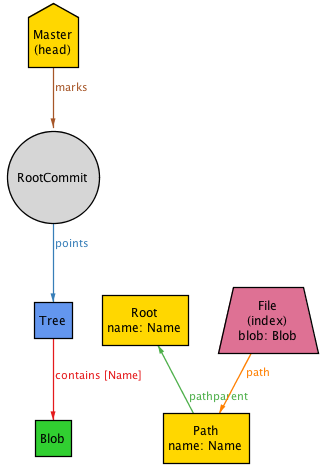
\includegraphics[width=0.8\textwidth]{images/commit1.png}
   \caption{Doing a commit}\label{fig:commit1}
\end{figure}
\begin{figure}[!t]
   \centering
   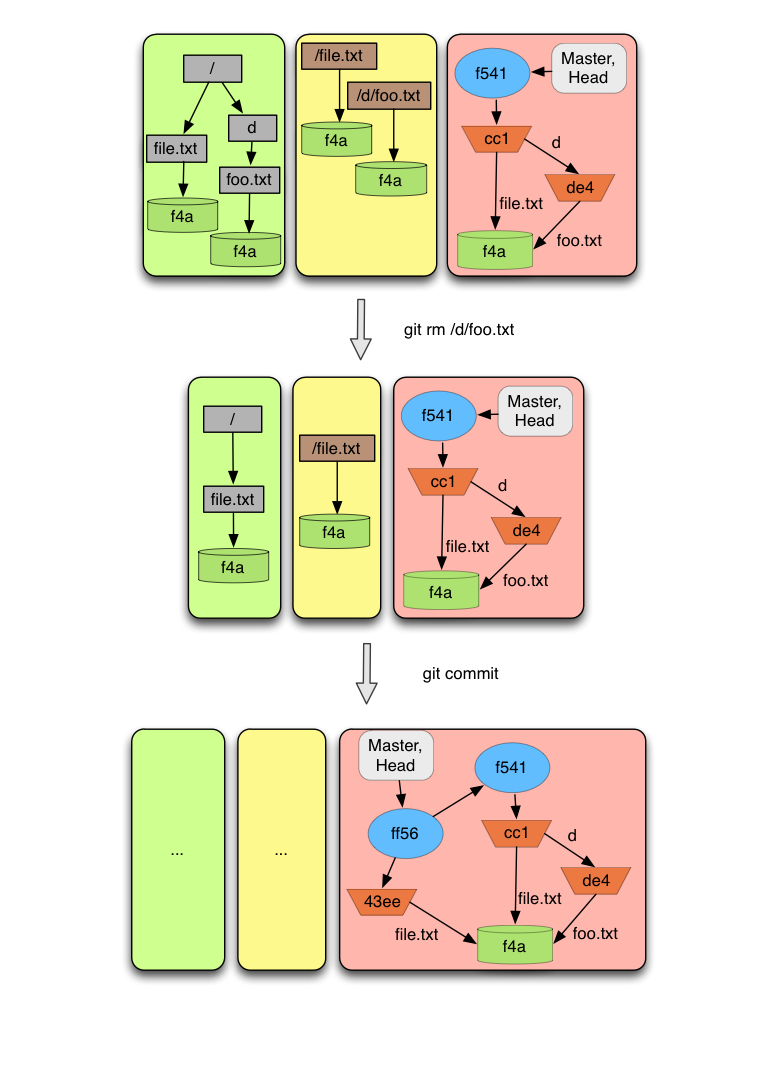
\includegraphics[width=0.8\textwidth]{images/commit2.png}
   \caption{Doing a second commit}\label{fig:commit2}
\end{figure}

\begin{figure}[!t]
   \centering
   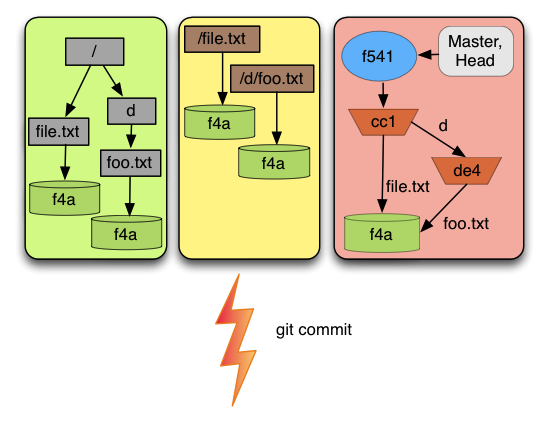
\includegraphics[width=0.6\textwidth]{images/commit_pre.png}
   \caption{This commit can't be done in \emph{git}}\label{fig:commit_pre}
\end{figure}

\subsection{Branch}

\subsubsection{Pre requisites}

\subsubsection{Result}

\subsubsection{Examples}
Git branch operation has several forms, that to different things on git.
The ones which we care are the forms that create and delete branches. \par
When a new branch is created it will point to the current HEAD by default.
\par


The man git-branch says that when deleting a branch, it must be fully
merged in its upstream branch, or in HEAD if no upstream was set. \par


\begin{figure}[!t]
   \centering
   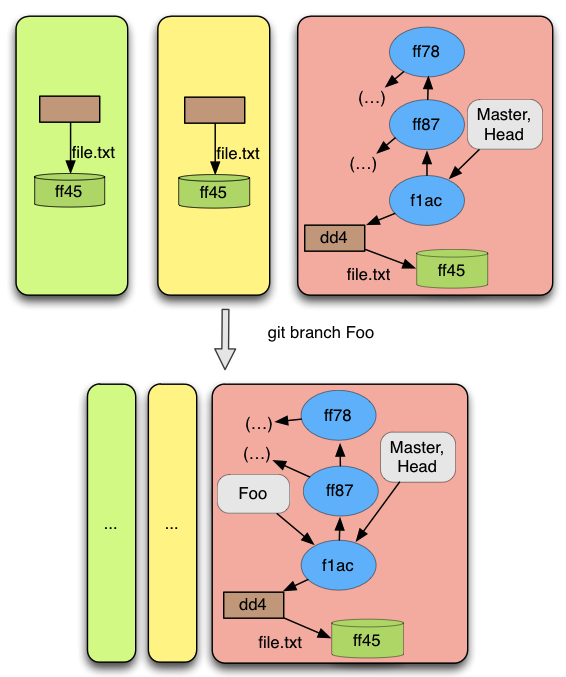
\includegraphics[width=0.6\textwidth]{images/branch.png}
   \caption{Creating a branch}\label{fig:branch}
\end{figure}

\subsection{Checkout}

\subsubsection{Pre requisites}

\subsubsection{Result}

\subsubsection{Examples}
From man git-checkout : "Switches branches by updating the index, 
working tree, and HEAD to reflect the specified branch or commit". \par
\begin{figure}[!t]
   \centering
   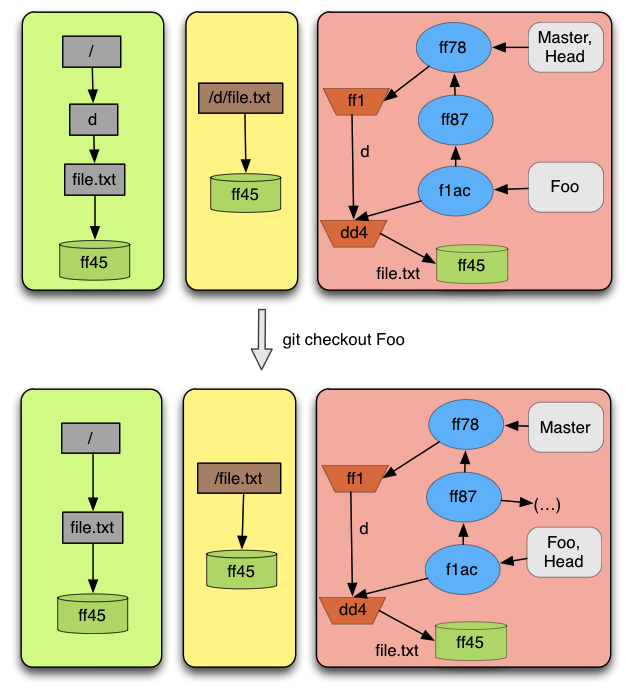
\includegraphics[width=0.6\textwidth]{images/checkout.png}
   \caption{A simple checkout}\label{fig:checkout}
\end{figure}

\subsection{Merge}


When you do a 'git merge <branch>', a merge will happen between the current
branch and the branch selected on the command. The result will be a new merge 
commit, or a partially merged index. \par

Git knows three types of merge : 
\begin{itemize}
\item A fast-forward merge, that will happen when 
the current commit from the other
branch, is more recent than the current commit from the current branch. \par
This type is not a true merge, in the sense that the only thing that
changes it's the pointer of the current branch
is moved to the newest commit.

\item A 2-way merge, that happens when the conditions for a fast-forward
don't exist, and there isn't a common ancestor for both commits.

\item A 3-way merge, happens when the conditions for a fast-forward
don't exist, but, there is a common ancestor for both commits. \par
The difference between these two last types, is that the last is much 
more automatic having much less conflicts than the previous type.
\end{itemize}
Knowing these 3 types of merge, it's important to know that Git tries to make
the merge process as automatic as possible. However conflicts do exist, and when
they happen it leaves to the user the process of resolving those conflicts. \par
When the Git/user, finishes the merging of files in the index, he
can commit the resulting merge, in a merge commit. \par
Note that while there are unmerged files in the index, a commit cannot be
made. \par 

\subsubsection{Pre requisites}

\begin{itemize}
\item A merge can't be made, if the current commit is more recent then the
other commit.
\item A merge can't be made, while there are unmerged files.
\item In the case of a fast-forward merge, the index can't have uncommitted
files that can be changed by the merge operation.
\item In the case of a 2-way or 3-way merge operation there can not be
uncommitted files. 
\end{itemize}

\subsubsection{Result}

\subsubsection{Examples}

\begin{figure}[!t]
   \centering
   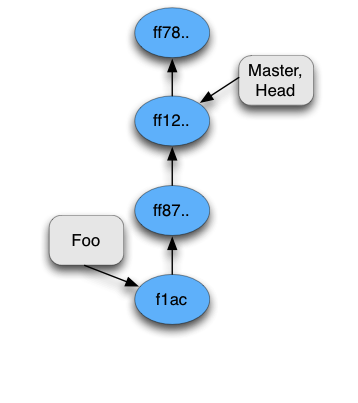
\includegraphics[width=0.5\textwidth]{images/fast_forward.png}
   \caption{A fast-forward case}\label{fig:fast_forward}
\end{figure}

\begin{figure}[!t]
   \centering
   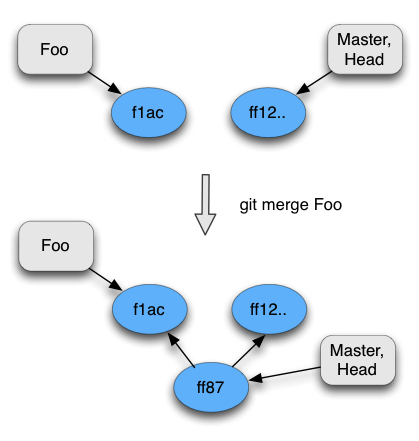
\includegraphics[width=0.6\textwidth]{images/2merge.png}
   \caption{A 2-way merge case}\label{fig:2mergecase}
\end{figure}

\begin{figure}[!t]
   \centering
   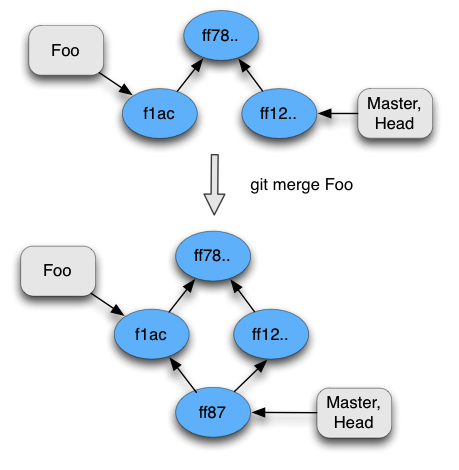
\includegraphics[width=0.6\textwidth]{images/3merge.png}
   \caption{A 3-way merge case}\label{fig:3mergecase}
\end{figure}

\begin{figure}[!t]
   \centering
   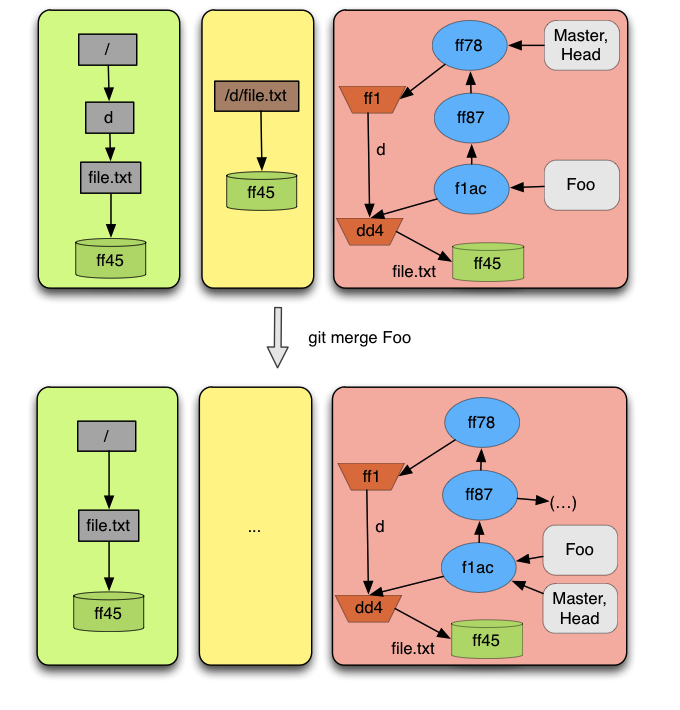
\includegraphics[width=0.6\textwidth]{images/fast_forward_merge1.png}
   \caption{A fast-forward merge case}\label{fig:ffmerge1}
\end{figure}

\begin{figure}[!t]
   \centering
   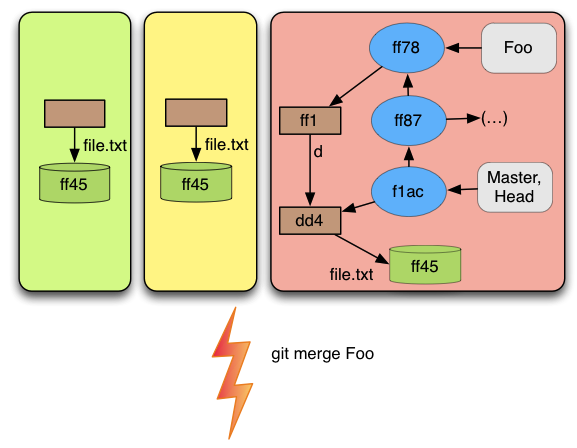
\includegraphics[width=0.6\textwidth]{images/fast_forward_merge_pre.png}
   \caption{A fast-forward case that can't be done in
   \emph{git}}\label{fig:ffmergepre}
\end{figure}

\begin{figure}[!t]
   \centering
   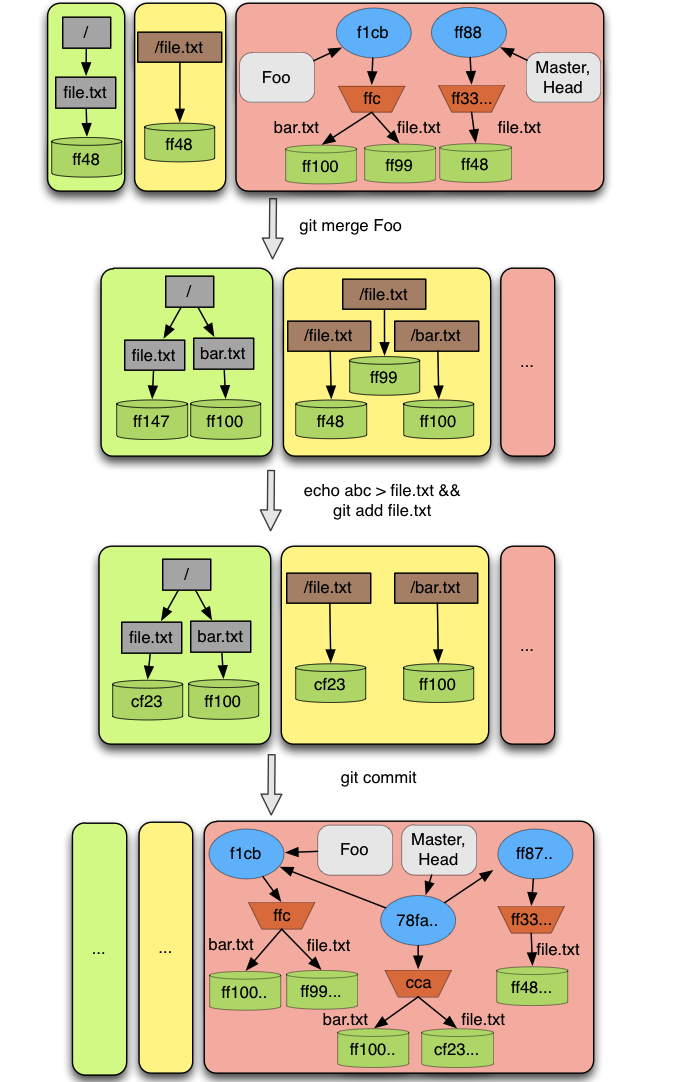
\includegraphics[width=0.7\textwidth]{images/merge2way}
   \caption{A typical 2-way merge}\label{fig:merge2way}
\end{figure}
\begin{figure}[!t]
   \centering
   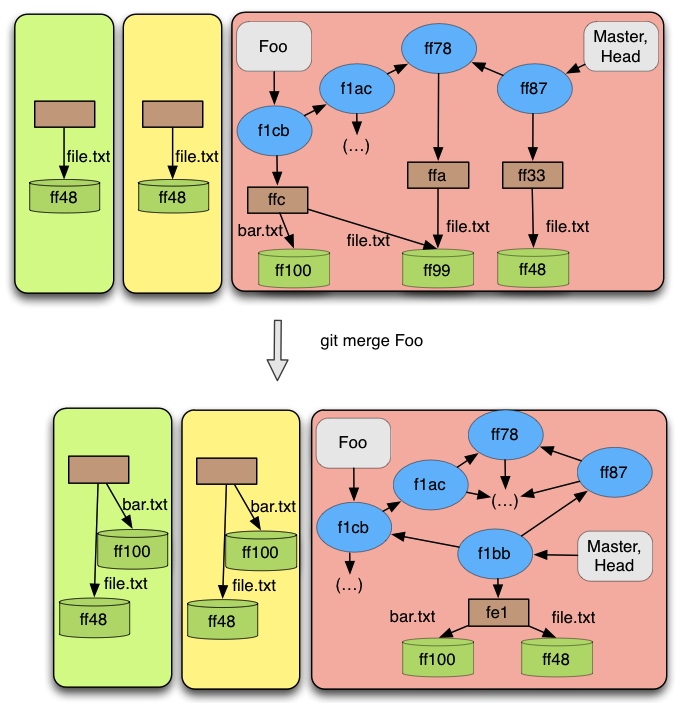
\includegraphics[width=0.7\textwidth]{images/merge3way}
   \caption{A typical 3-way merge}\label{fig:merge3way}
\end{figure}

\subsubsection{Git Pull and Git Push}

When working with remote repositories, these two operations will be vastly
used. They are in fact a sequence of operations, and are used to get content
from a remote repository and to place your content on the remote repository.
\par
If a 'git pull' is done, the branch from the remote repository will be fetched,
and the local branch and the remote branch will be merged. \par
If a 'git push' is done, the remote branch will be uploaded to the remote 
repository and will be merged there. \par
However, a 'git push' can only be done when the resulting merge will be a
fast-forward, simply because there is no one on the other side to resolve the 
merge conflicts. For the case of 'git pull' it's pre requisites are the same of
the merge operation. \par
